% siminos/gudorf/thesis/chapter/numerics.tex
% $Author: predrag $ $Date: 2020-10-24 01:45:26 -0400 (Sat, 24 Oct 2020) $


In our Newton methods we measure the distance of the guess to the solution
by Euclidian sums of squares.

In discrete {Lagrangian} methods the distance between a guess solution and
the exact solution is measured in the symplectic area between the two.

Lagrangian:
\(
L(q,\dot{q})=K(\dot{q})-V(q)
\)

Action:
\(
S(q)=\int_0^T \!dt L(q,\dot{q})
\)

Hamilton's principle:
\(
\delta S(q)=0
\)

if we vary the path slightly, action is
unchanged to first order.

%%%%%%%%%%%%%%%%%%%%%%%%%%%%%%%%%%%%%%%%%%%%%%%%%%%%%%%%%%%%%%%
  \begin{figure}
  \begin{center}  %%% 2016-12-25  see
                  %%% siminos/figsSrc/inkscape/CatMapStatesp.svg
  \setlength{\unitlength}{0.45\textwidth}
 %% \unitlength = units used in the Picture Environment
  \begin{picture}(1,0.42749291)%
    \put(0,0){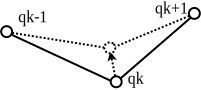
\includegraphics[width=\unitlength]{DiscrLagrVar}}%
    \put(0.77112773,0.37243164){\color[rgb]{0,0,0}\makebox(0,0)[lb]{\smash{$\ssp_{k+1}$}}}%
    \put(0.08972224,0.32911934){\color[rgb]{0,0,0}\makebox(0,0)[lb]{\smash{$\ssp_{k-1}$}}}%
    \put(0.63560716,0.022384){\color[rgb]{0,0,0}\makebox(0,0)[lb]{\smash{$\ssp_{k}$}}}%
  \end{picture}%
\end{center}
   \caption{ \label{fig:DiscrLagrVar}
%(Color online)
Discrete Euler-Lagrange equations are an extremum of the action.
   }
 \end{figure}
%%%%%%%%%%%%%%%%%%%%%%%%%%%%%%%%%%%%%%%%%%%%%%%%%%%%%%%%%%%%%%%%

The variational principle: path extremizes action

Discrete treatment of
Lagrangian mechanics:

Approximate action integral by a quadrature
rule
\[
L(q_k,q_{k+1}) \approx \int_{t_k}^{t_{k+1}} L(q,\dot{q})\,dt
    =
{\Delta t} L(q_k,q_{k+1})
\,.
\]


Symplecticity:
If we graph trajectories in the phase plane,
symplectic methods preserve areas in time.
This means that a closed loop (e.g. a periodic
motion, like the pendulum) won't expand or
contract.

The Legendre transforms between different generating function are of form
\[
H(q_k,p_{k+1})=p_{k+1}q_{k+1}-L(q_k,q_{k+1})
\,,
\]
where $q_{k+1}$ is implicitly defined by $p_{k+1}=\partial_2 L(q_{k},q_{k+1})$

Search for:

Asynchronous variational integrators (AVI). They assign different time
steps at different points in space (where more/less accuracy is
needed).

Example: falling object

Discrete Lagrangian:
\[
L(q_k,q_{k+1}) =
{\Delta t} \left[
\frac{1}{2} m \left(\frac{q_{k+1}-q_k}{{\Delta t}}\right)^2
- mg \left(\frac{q_k+q_{k+1}}{2}\right)^2
  \right]
\,.
\]
Discrete Euler-Lagrange equations
\beq %\label{eq:Definition generating function compound map}
\frac{\partial}{\partial q_{n}}
    \left( \genF(q_{n-1},q_{n}) + \genF(q_{n},q_{n+1}) \right)=0
    \,.
\ee{MKMP84(3.7)a}
lead to
\[
-m\,\frac{q_{k+1}-q_k}{{\Delta t}} - \frac{1}{2} {\Delta t}\,mg
+ m\,\frac{q_k-q_{k-1}}{{\Delta t}} - \frac{1}{2} {\Delta t}\,mg
        =0
\,.
\]
hence,
writing the acceleration as s discrete time Laplacian, the falling
object equation is
\bea
\frac{1}{{\Delta t}^2}\Box\,\ssp_n
    &=& -g
\continue
\Box\,\ssp_n &\equiv& \ssp_{n+1} - 2\,\ssp_{n} + \ssp_{n-1}
    \label{LaplTime}
\,.
\eea

Adding forcing/dissipation

For non-conservative forces, use the discrete Lagrange d'Alembert principle
by varying the {\em action}
    \beq %\label{eq:Definition generating function compound map}
\delta \action_{n,n+k} + \sum_{i=n}^{n+k-1}
\left(
F^{-}(q_{i},q_{i+k})\,\delta q_k
     +
F^{+}(q_{i},q_{i+k})\,\delta q_{k+1}
\right)
\,,
    \ee{MKMP84(3.5)a}
This gives the forced discrete Euler-Lagrange equations
\beq %\label{eq:Definition generating function compound map}
\frac{\partial}{\partial q_{n}}\genF(q_{n-1},q_{n})
 +
\frac{\partial}{\partial q_{n}}\genF(q_{n},q_{n+1})
 +
F^{-}(q_{i},q_{i+k})
 +
F^{+}(q_{i},q_{i+k})
=0
    \,.
\ee{MKMP84(3.7)b}
This is then illustrated by two strengths of frictional (linear
in velocity) damping of a damped pendulum.

\subsection{Literature survey}
\label{sect:spatioTempNumer}

\begin{description}
\item[2018-03-28 PC]

\HREF{https://hoj201academic.wordpress.com/} {Henry O. Jacobs}
course notes
\HREF{https://hoj201academic.files.wordpress.com/2012/09/hoj_disc_lag_mech_tut.pdf}
{Crash course in discrete {Lagrangian} mechanics}\rf{Jacobs12}
are in their entirety based on Marsden and West\rf{MarWes01} {\em Discrete
mechanics and variational integrators}, which has some 600 citations, so ther
is a large amount of literature to scan through.

Eva Kanso says that the discrete {Lagrangian} integration is formulated for
Euler in Pavlov\rf{PMTKMD11} {\em Structure-preserving discretization of
incompressible fluids}, \arXiv{0912.3989}, but if it works, it should also
work for Navier-Stokes by ``modelling the dissipation.''
They write: ``
Euler fluids have Lagrangian and
Hamiltonian descriptions, where the configuration space is
defined as the volume-preserving diffeomorphisms, and Kelvin's circulation
theorem is viewed as a consequence of Noether's theorem associated with the
particle relabeling symmetry of fluid mechanics. However computational
approaches to fluid mechanics have been largely derived from a
numerical–analytic point of view, and are rarely designed with structure
preservation in mind, and often suffer from spurious numerical artifacts such
as energy and circulation drift. In contrast, this paper geometrically
derives discrete equations of motion for fluid dynamics from first principles
in a purely Eulerian form. Our approach approximates the group of
volume-preserving diffeomorphisms using a finite-dimensional Lie group, and
associated discrete Euler equations are derived from a variational principle
with non-holonomic constraints. The resulting discrete equations of motion
yield a structure-preserving time integrator with good long-term energy
behavior and for which an exact discrete Kelvin's circulation theorem
holds.

[...] understanding  what  this  geometric  picture  of  fluid  flows brings
compared to traditional Large Eddy Simulation or Reynolds-Averaged
Navier-\-Stokes methods would be interesting, as our structure-preserving
approach is also based on local averages (i.e., integrated values) of the
velocity field.


The discretization of the Euler equations that we have obtained on the
regular grid coincides with the Harlow-Welsh scheme\rf{HarWel65}, and our Eq.
(28) is a Crank-\-Nicolson (trapezoidal) time update.  Therefore, our
variational scheme can be seen as  an  extension  of  this  approach  to
arbitrary  grids,  offering  the  added  bonus  of providing a geometric
picture.
''


\item[2018-03-29 Evangelos]
Good people to ask about such methods might be
Cristel Chandre or Phil Morrison.

\item[2018-03-30 PC]
Cristel is a regular visitor, but it is all about Dirac brackets - not sure
it helps for dissipative flows. I think it is the same / similar story for
Phil. But we can ask - Jeffrey Heninger is now his PhD student.

\begin{figure}
\centering
    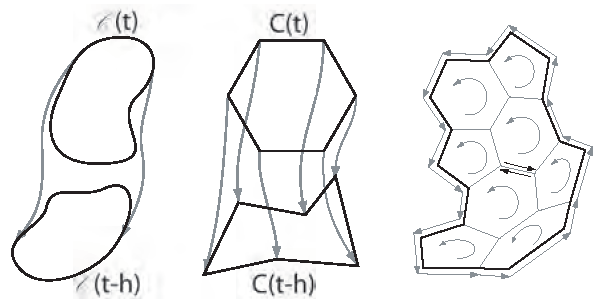
\includegraphics[width=.75\textwidth]{GDPSS06fig5}
\caption{\label{fig:GDPSS06fig5}
Kelvin's Theorem: (left) in the continuous setting, the circulation
on any loop being advected by the flow is constant. (middle) the discrete
integration scheme enforces this property on each Voronoi loop, (right) thus
on any discrete loop. (Fig.~5 on page~63 ofn \refref{GDPSS06})
        }
\end{figure}


\item[2018-03-30 PC] Eva Kanso  sent us Grinspun \etal\rf{GDPSS06}
{\em Discrete Differential Geometry: An Applied Introduction} set of coure=se
notes to read. Presumably we should read {\em Discrete differential forms for
computational modeling}, which is a mostly mathematical discussion of
``discrete differential modeling,'' which I intend to skip, unless really
forced to learn it. {\em Stable, circulation-preserving, simplicial fluids}
is perhaps more relevant:

`` the approach also provides an accurate treatment of vorticity through a
discrete preservation of Kelvin's circulation theorem.''

The code, however, for all examples discussed, is spatial, and steps forward in time.

``
For purposes of computation one must derive discrete (in space and time)
representations of the underlying equations. The theories, which are discrete
from the start, and have key geometric properties built into their discrete
description can often more readily yield robust numerical simulations which
are true to the underlying continuous systems: they exactly preserve
invariants of the continuous systems in the discrete computational realm.

Jos Stam [1999; 2001] introduced to the graphics community the method of
characteristics for fluid advection and the Helmholtz-Hodge decomposition to
ensure the divergence-free nature of the fluid motion [Chorin and Marsden
1979].

Discrete exterior calculus (DEC) leads to numerically robust and efficient
simulations of the Navier-Stokes equations.
''

``
Fluid simulation are rarely designed to conserve defining physical
properties. Consider, for example, the need in many methods to continually
project the numerically updated velocity field onto the set of divergence
free velocity fields; or the need to continually reinject vorticity lost due
to numerical dissipation as a simulation progresses. We describe a
geometry-based algorithm for fluid simulation which exactly preserves
vorticity at a discrete level.

A careful setup of discrete differential quantities, designed to respect
structural relationships such as vector calculus identities, leads to a
numerical simulation method which respects the defining geometric structure
of the fluid equations.

We construct an integration scheme which employs intrinsically
divergence-free variables, and removes the need to enforce the usual
divergence-free constraint through a numerically lossy projection step.

The fundamental idea of geometric integration algorithm is to ensure that
Kelvin's theorem holds in the discrete setting: the circulation around any
loop in the fluid remains constant as the loop is advected,
see \reffig{fig:GDPSS06fig5}.
''

\item[2018-04-27 Samuel Hadden]
A widely used method for integrating multi-planet systems is
 Wisdom and Holman\rf{WisHol91}, see also discussion of it in Wisdom\rf{Wisdom17}.

Tsang \etal\rf{TGST15} generalize symplectic integration to treat
dissipative forces, \arXiv{1506.08443}

\item[2018-04-27 Noah DeTal, Predrag]
\HREF{https://scholar.google.com/citations?hl=en&user=4znehJIAAAAJ}
{Michael Kraus} is a busy beaver, developing variational integrators
for MHD.

Kraus and Maj\rf{KraMaj15}
{\em Variational integrators for nonvariational partial differential equations}
seems to be one of the most recent treatments with
all features we talked about: variational / Lagrangian formulation,
enforcement of conserved quantities / incompressibility, and applicability to
viscous / dissipative systems.

It's quite interesting - it imposes the constraint of satisfying the equations
of motion locally as we always do, by a Lagrangian multiplier. But then one
gets quite a bit of milage out of that matter of fact statement.

Kraus works with Phil Morrison, and by extension with Jeffrey Heninger, who
is currently his PhD student, see {\bf 2018-03-29 Evangelos} remark above.
They presented a 2017 poster titled {\em First numerical results towards a 3D
MHD equilibrium solver via artificial relaxation mechanisms }, but I do not
see a published version yet.

They say:

Embed an arbitrary dynamical system into a larger
Lagrangian system using the method of formal (or adjoint) Lagrangians, and
thereby extend the application domain of variational integrators to include
all dynamical systems.

To obtain a formal Lagrangian L, the equation $F [u] = 0$ is multiplied by an
adjoint variable $v$, giving $L = v \cdot F[u]$. Variation of the resulting
action functional $A = \int  d^{n+1}x L$ with respect to $v$ recovers the
original equation $F [u] = 0$. Variation of the action functional with
respect to the physical variable $u$ gives an additional equation that
determines the evolution of the adjoint variable $v$.

The dynamics of $v$ play a key role in relating symmetries of the formal
Lagrangian to conservation laws satisfied by $u$. Ibragimov\rf{Ibragimov06,
Ibragimov07a, Ibragimov07b} developed conservation laws of arbitrary
differential equations by extending the Noether theorem to formal Lagrangians
for the extended system $(u, v)$, which can be restricted to the original
system provided that it is possible to express the solution of the adjoint
variable $v$ in terms of $u$.

About Ibragimov: see
\HREF{http://gammett.ugatu.su/index.php?option=com_content&view=article&id=329\%3Anail-h-ibragimov&catid=66\%3Astaff-description&Itemid=130}
{here},
\HREF{http://www.bth.se/alga}{ALGA}, and his
\HREF{http://gammett.ugatu.su/index.php?option=com_content&view=category&layout=blog&id=11&Itemid=29}
{collected works}.
Further articles to check out:

Ibragimov\rf{Ibragimov11}
{\em Nonlinear self-adjointness and conservation laws}: ``
The general concept of nonlinear self-adjointness of differential
equations is introduced. It  embraces the strict self-adjointness
and quasi-self-adjointness. The equations possessing nonlinear
self-adjointness can be written equivalently in a strictly self-adjoint
form by using appropriate multipliers. All linear equations possess the
property of nonlinear self-adjointness, and hence can be rewritten in a
nonlinear strictly self-adjoint form.
''

Ibragimov\rf{Ibragimov18} {\em Conservation laws and non-invariant solutions
of anisotropic wave equations with a source}.

The good news is the Ibragimov is a triviality, says Anco\rf{Anco17} {\em
On the incompleteness of {Ibragimov}'s conservation law theorem and its
equivalence to a standard formula using symmetries and
adjoint-symmetries}

Then come along Ruggieri and Speciale\rf{RugSpe17}
{\em Conservation laws by means of a new mixed method}, and,
citing but ignoring Anco's contemporaneous gripe,
``merge the Ibragimov's method and the 1966 one by Anco and Bluman.''

\item[2019-04-17 Predrag]
Wei and Wang\rf{WeiWan19} {\em Symmetry analysis, conserved quantities and
applications to a dissipative {DGH} equation} describe and utilize Ibragimov's
approach:

``
Sophus Lie introduced the notion of Lie group in order to study the solutions of
ordinary differential equations. He showed
that the order of an ordinary differential equation can be reduced if it is
invariant under one-parameter Lie group of point transformations. The
applications of Lie groups to differential systems were mainly established by Lie
and Emmy Noether. In 1918, Noether presented the relationship between a
mathematics symmetry and conservation law of a physical system. Noether's (first)
theorem states that every differentiable symmetry of the action of a physical
system has a corresponding conservation law.
[...]

Noether's theorem can only be applied to equations with variational structure. A
large number of differential equations without variational structure admit
conservation laws. Thus, many authors developed some methods which do not rely on
the knowledge of Lagrangian functions to obtain conservation laws, such as the
characteristic method\rf{liede} and the direct method\rf{AncBlu02I,AncBlu02II}.
Ibragimov\rf{Ibragimov07a} proved a result which allows one to construct
conservation laws for equations without variational structure. Ibragimov theorem
is an extension of Noether's theorem where a formal Lagrangian is introduced in
order to get rid of the variational limitation. This paper uses the viewpoint of
Lie symmetry analysis to construct conservation laws by Ibragimov's theorem in
this paper.

They start by presenting the notations, definition of nonlinear self-adjointness
and Ibragimov's theorem on conservation laws. Next, they carry out Lie symmetry
analysis, derive some symmetry reductions and invariant solutions for their
system, a dissipative {DGH} equation. They then study the self-adjointness and
conservation laws of DGH by the Ibragimov's theorem.
''

\item[2019-05-21 Predrag]
\HREF{https://scholar.google.com/citations?user=lVixLdgAAAAJ}
{Mikhail Skopenkov}
(smart cookie; for slides, see \HREF{http://skopenkov.ru/}{skopenkov.ru})
{\em Discrete field theory: symmetries and conservation laws}\rf{Skopenkov17},
\arXiv{1709.04788}, gives ``a general algorithm constructing a discretization
of a classical field theory from a Lagrangian, with a discrete Noether
theorem relating symmetries to conservation laws and an energy conservation
theorem not based on any symmetry. This gives exact conservation laws for
electrodynamics, gauge theory, Klein-Gordon
and Dirac theory. He constructs a conserved discrete
energy-momentum tensor, approximating the continuum one at least for free
fields. The theory is stated in topological terms, such as coboundary and
products of cochains.''

His \emph{principles of discretization} are:
\begin{itemize}
\item keep approximation of continuum theory;
\item keep conservation laws exact;
\item drop spatial symmetries easily.
\end{itemize}
He obtains:
\begin{itemize}
\item
    discretization of several field theories in a similar fashion keeping
    conservation laws exact;
\item
    a discrete Noether theorem relating symmetries to conservation laws;
\item
    a discrete energy conservation theorem not based on a symmetry.
\end{itemize}

\item[2019-11-05 James Hanna] <hannaj@vt.edu> from
\HREF{http://www2.esm.vt.edu/~hannaj/} {Virginia Tech} writes:
Could you please point me to the discrete Noether business you referred to?

\HREF{https://ce.gatech.edu/node/421}
{Arash Yavari} is an interesting neighbor of yours.
He has been teaching at GaTech since 2005. He studies computational mechanics, and
in particular has been working to develop systematic theories of discrete
mechanics for crystalline solids with defects.

Here is something else interesting:

Gay-Balmaz and Yoshimura\rf{GayYos17a} {\em A {Lagrangian} variational
formulation for nonequilibrium thermodynamics. {Part I: Discrete} systems}, early
version \arXiv{1510.00792}

Gay-Balmaz and Yoshimura\rf{GayYos17} {\em A free energy {Lagrangian}
variational formulation of the {Navier-Stokes-Fourier} system},
\arXiv{1706.09010}

\item[2019-11-06 Predrag] More of such, some of it impossible to read:

Scholle and F. Marner\rf{SchMar17}
{\em A non-conventional discontinuous {Lagrangian} for viscous flow},
also \HREF{https://core.ac.uk/reader/84153262} {here}
looks quite interesting, and perhaps even implementable: ``
In an analogy with Madelung quantum mechanical fluid, a new Lagrangian is
proposed for a variational formulation of the Navier–Stokes equations.
''


Gay-Balmaz and Yoshimura\rf{GayYos18} {\em Dirac structures in nonequilibrium
thermodynamics}, \arXiv{1704.03935}: ``
In absence of irreversible processes these Dirac structures reduce to canonical
Dirac structures associated to canonical symplectic forms on phase spaces. Our
geometric formulation of nonequilibrium thermodynamic thus consistently extends
the geometric formulation of mechanics, to which it reduces in absence of
irreversible processes.
''

Gay-Balmaz and Yoshimura\rf{GayYos18a} {\em Variational discretization of the
nonequilibrium thermodynamics of simple systems}, \arXiv{1601.04882}: ``
[...] extend the variational integrators of Lagrangian mechanics to include
irreversible processes. The structure preserving property of the flow of such
systems is an extension of the symplectic property of the flow of the
Euler–Lagrange equations. In the discrete setting, we show that the discrete flow
solution of our numerical scheme verifies a discrete version of this property.
''

Bourdin \etal\rf{BCGI16} {\em Variational integrators of fractional {Lagrangian}
systems in the framework of discrete embeddings},  \arXiv{1601.04882}: ``
[...] interested in the conservation at the discrete level of this Lagrangian
structure by discrete embeddings. We then replace in this framework the
variational integrators developed in [Hairer \etal\rf{HaLuWa06}, Chapter VI.6,
\CBlibrary{HaLuWa06}] and
Marsden and West\rf{MarWes01}.

Not directly related, but
I liked Harmeet Singh and J. Hanna {\em Impulse and material symmetry}
APS DFD talk at Virginia Tech
(Jean-Luc Thiffeault would like it too, I think): ``
The balance of material momentum, also known as impulse or pseudomomentum, arises
from material (relabeling) symmetry. We will present a brief overview of the
history of this balance law of continuum mechanics, and discuss it in the context
of an ideal fluid. It will be shown that Kelvin's circulation theorem, Cauchy's
invariants, Weber's integral, and other related quantities follow from this
balance law
''

\end{description}

\section{Noether's theorem}
\label{sect:NoetherThe}


\begin{description}
    \PCpost{2016-11-23}{
A variational principle (such as the action \refeq{GutOsi15-3.1:model} in case
at hand) together with a continuous symmetry implies
\begin{quote}
\textbf{Noether's
theorem}: To every one-parameter, continuous group of symmetries of a Lagrangian
dynamical system there corresponds a scalar, real-valued conserved quantity.
\end{quote}
Is there is a version of it for discrete translations? What is the conserved
quantity for a single cat map? What is it for the lattice? Internet says
many contradictory things:

``The fact that a Lagrangian is unchanged by a discrete transformation  is of
no significance. There is no conserved quantity associated with the
transformation.''

``For infinite symmetries like lattice translations the conserved quantity is
continuous, albeit a periodic one. So in such case momentum is conserved
modulo vectors in the reciprocal lattice. The conservation is local just as
in the case of continuous symmetries.''

Read about it
\HREF{http://physics.stackexchange.com/questions/8518/is-there-something-similar-to-noethers-theorem-for-discrete-symmetries}
{here}.

{Mansfield}\rf{Mansfield06} in proceedings
\HREF{https://www.kent.ac.uk/smsas/personal/elm2/liz/papers/focm.pdf}
{here} and in her
\HREF{https://www.kent.ac.uk/smsas/personal/elm2/liz/papers/santander-land.pdf} {talk}
defines \emph{total difference} and says ``
Just as an integral of a total divergence depends only on the boundary data,
so does the sum over lattice domain of a total difference.''

She states the discrete {Noether's} Theorem, and in her Example 1.3.7  she shows
that for a discretization of a standard mechanical Lagrangian, time
invariance yields ``energy'' as a the conserved quantity.

Hydon and Mansfield\rf{HydMan11}.

Capobianco and Toffoli\rf{CapTof11} {\em Can anything from {Noether's} Theorem be
salvaged for discrete dynamical systems?} is fun to read (but ultimately
unsatisfactory):

``
we take the Ising spin model with both
ferromagnetic and antiferromagnetic bonds. We show that --and why--
energy not only acts as a generator of the dynamics for this family of
systems, but is also conserved when the dynamics is time-invariant.''

The \emph{microcanonical Ising model} is strictly deterministic and
invertible: on a given step, a spin will flip (that is, reverse its
orientation) if and only if doing so will leave the sum of the potential
energies of the four surrounding bonds unchanged. The Ising dynamics is a
second-order recurrence relation. They define ``energy'' as the length of the
boundary between `up' and `down' domains. While the magnetization—number of
spins up minus number of spins down—may change with time, that length, and
thus the energy, remains constant. The total energy of a system may be
defined as
\begin{enumerate}
  \item A real-valued function of the system's state,
  \item that is additive,
  \item and is a generator of the dynamics.
\end{enumerate}
In a discrete Hamiltonian dynamics, a state is no longer a
``position / momentum'' pair $<q,p>$ as in the continuous case, but an ordered
pair of configurations $<q_0,q_1>$.

A second-order dynamical system
has an evolution rule of the form
\[
x_{t+1} = g(x_{t},x_{t-1})
\,.
\]
            }

\end{description}
